\documentclass[11pt,a4paper,oneside]{book}	% definition book
\usepackage[utf8x]{inputenc}				% encoding
\usepackage[T1]{fontenc}    				% hyphenation special chars
%\usepackage[ngerman]{babel}				% German grammar rules
\usepackage[english]{babel}					% English grammar rules
\usepackage{ucs}							% extended utf-8 support
\usepackage{amsmath}						% writing math formulas
\usepackage{amsfonts}						% math fonts
\usepackage{amssymb}						
\usepackage{makeidx}
\usepackage{showidx}
\usepackage[dvips]{graphicx}           		% to include images
\usepackage{pslatex}	    				% to use PostScript fonts

%
% Command
%

\newcommand{\HRule}{\rule{\linewidth}{0.5mm}}

% ==================================================================
% General Settings
% ==================================================================

\makeindex

% ==================================================================
% Document
% ==================================================================

\begin{document}
% ----------------------------------
% front
% ----------------------------------
\frontmatter								% roman numerals for page numbers
\begin{titlepage}

\begin{center}

% Upper part of the page
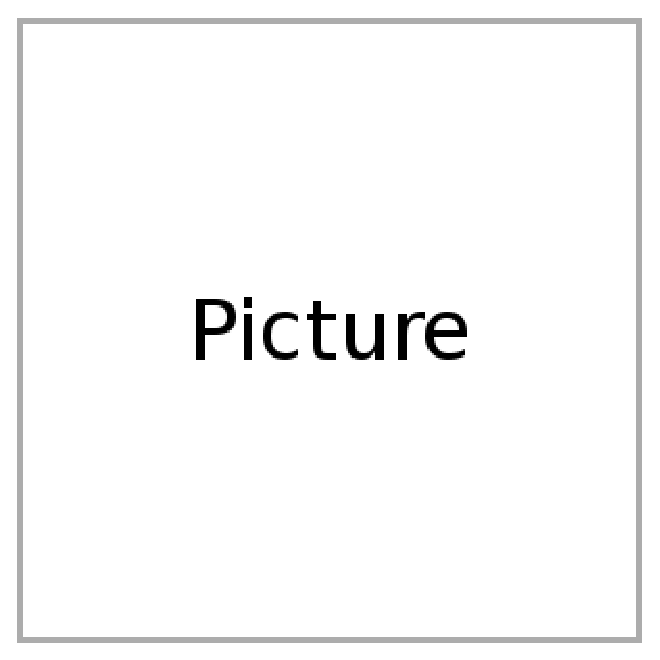
\includegraphics[width=0.5\textwidth]{img/picture}\\[1cm]    
\textsc{\LARGE ANYTHING}\\[1.5cm]

% Title
\HRule \\[0.4cm]
{ \huge \bfseries TITLE OF THIS BOOK}\\[0.4cm]
\HRule \\[1.5cm]
\textsc{\Large SUB DESCRIPTION}\\[0.5cm]

\vfill

% Bottom of the page
\author{AUTHOR}
{\large \today}

\end{center}
\end{titlepage}
\tableofcontents
\listoffigures
\listoftables

% ----------------------------------
% main
% ----------------------------------
\mainmatter									% chapter numbering

\part{Examples}
\chapter{Simple Image Chapter}

\begin{figure}[htp] % h .. float, t .. top
	\centering
	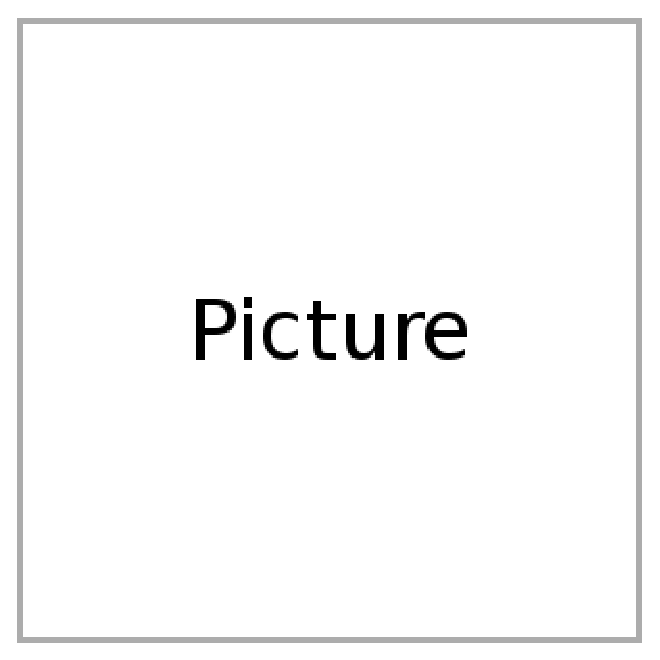
\includegraphics[width=150px]{img/picture}
	\caption{Simple Image Caption}
\end{figure}

\section{Section}

We cite from A.S.~\cite[p.~48]{book00}

\subsection{Subsection}

% ----------------------------------
% appendix
% ----------------------------------
\appendix

% ----------------------------------
% back
% ----------------------------------
\backmatter
% add literature list to table of contents
\addcontentsline{toc}{part}{Literature}
% show literature list
\bibliographystyle{alpha}
\bibliography{book}

\end{document}